\documentclass[12pt,a4paper]{article}
\usepackage[utf8]{inputenc}
\usepackage[russian]{babel}
\usepackage{graphicx}
\usepackage{wrapfig}
\usepackage{calc}
\usepackage{picinpar}
%\usepackage{floatflt}

\newcommand{\myfig}[2][0.43]{
\begin{wrapfigure}{l}{0pt}
\includegraphics[width=#1\textwidth]{#2}
\end{wrapfigure}
}

\newcommand{\myfigr}[2][0.43]{
\begin{wrapfigure}{r}{0pt}
\includegraphics[width=#1\textwidth]{#2}
\end{wrapfigure}
}

\begin{document}

%~ \newcounter{mywidth}
%~ \setcounter{mywidth}{}

\newlength\firstcolumnwidth
\newlength\secondcolumnwidth
\setlength\tabcolsep{0pt}

\newcommand\twocolumns[3]{
    \setlength\firstcolumnwidth{#1\textwidth}
    \setlength\secondcolumnwidth{\textwidth - \firstcolumnwidth - \tabcolsep - \tabcolsep}
    \begin{figure}[h]
    \begin{tabular}{p{\firstcolumnwidth} p{\secondcolumnwidth}}
    \vspace{1pt} #2 & #3 \\
    \end{tabular}
    \end{figure}
}





\section{Преподобный Силуан Афонский}


%~ \setlength\firstcolumnwidth{0.33\linewidth}
%~ 
%~ \setlength\secondcolumnwidth{\linewidth - \firstcolumnwidth - 0.01\linewidth}
%~ 
%~ \begin{figure}[h]
%~ \begin{minipage}[b]{\firstcolumnwidth}
%~ 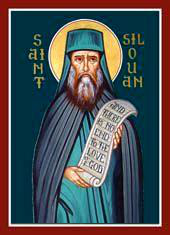
\includegraphics[width=\linewidth]{img/521.jpg}
%~ \end{minipage}
%~ \hspace{0.01\linewidth}
%~ \begin{minipage}[b]{\secondcolumnwidth}
%~ Будущий старец Силуан родился в крестьянской семье Тамбовской губернии в 1866 году, Призванный на военную службу в Петербург, он «умом пребывая на Афоне и на Страшном Суде», получает у св. праведного Иоанна Кронштадтского благословение на монашеский подвиг и в 1892 году становится послушником русского Пантелеимонова монастыря на Афоне. 
%~ 
%~ Монашеские подвиги преподобного Силуана были тайными, но особую благодать, которая от него исходила, чувствовали все, от простых рабочих до церковных иерархов. 
%~ 
%~ \end{minipage}
%~ 
%~ \end{figure}


\twocolumns{0.33}{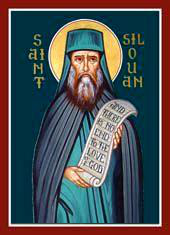
\includegraphics[width=0.33\textwidth]{img/521.jpg}}{
Будущий старец Силуан родился в крестьянской семье Тамбовской губернии в 1866 году, Призванный на военную службу в Петербург, он «умом пребывая на Афоне и на Страшном Суде», получает у св. праведного Иоанна Кронштадтского благословение на монашеский подвиг и в 1892 году становится послушником русского Пантелеимонова монастыря на Афоне.

Монашеские подвиги преподобного Силуана были тайными, но особую благодать, которая от него исходила, чувствовали все, от простых рабочих до церковных иерархов. 

}

После смерти старца, последовавшей в 1938 году, в Пантелеимонов монастырь стали приходить многочисленные письма, свидетельствующие о его небесном предстательстве за тех, кто обращался к нему с молитвой.

\section{Преподобный Силуан Афонский}


%~ \setlength\firstcolumnwidth{0.33\linewidth}
%~ 
%~ \setlength\secondcolumnwidth{\linewidth - \firstcolumnwidth - 0.01\linewidth}
%~ 
%~ \begin{figure}[h]
%~ \begin{minipage}[b]{\firstcolumnwidth}
%~ 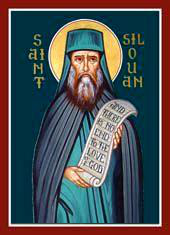
\includegraphics[width=\linewidth]{img/521.jpg}
%~ \end{minipage}
%~ \hspace{0.01\linewidth}
%~ \begin{minipage}[b]{\secondcolumnwidth}
%~ Будущий старец Силуан родился в крестьянской семье Тамбовской губернии в 1866 году, Призванный на военную службу в Петербург, он «умом пребывая на Афоне и на Страшном Суде», получает у св. праведного Иоанна Кронштадтского благословение на монашеский подвиг и в 1892 году становится послушником русского Пантелеимонова монастыря на Афоне. 
%~ 
%~ Монашеские подвиги преподобного Силуана были тайными, но особую благодать, которая от него исходила, чувствовали все, от простых рабочих до церковных иерархов. 
%~ 
%~ \end{minipage}
%~ 
%~ \end{figure}


\begin{window}[0,l,{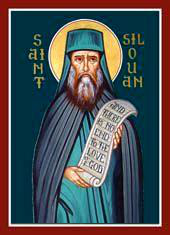
\includegraphics[width=0.33\linewidth]{img/521.jpg}},{}]
Будущий старец Силуан родился в крестьянской семье Тамбовской губернии в 1866 году, Призванный на военную службу в Петербург, он «умом пребывая на Афоне и на Страшном Суде», получает у св. праведного Иоанна Кронштадтского благословение на монашеский подвиг и в 1892 году становится послушником русского Пантелеимонова монастыря на Афоне.

\par Монашеские подвиги преподобного Силуана были тайными, но особую благодать, которая от него исходила, чувствовали все, от простых рабочих до церковных иерархов. 



%~ \parindent



После смерти старца, последовавшей в 1938 году, в Пантелеимонов монастырь стали приходить многочисленные письма, свидетельствующие о его небесном предстательстве за тех, кто обращался к нему с молитвой.
\end{window}

%~ \newpage\section{test}
%~ 
%~ \begin{floatingfigure}[l]{0.2\textwidth}
%~ \centering
%~ 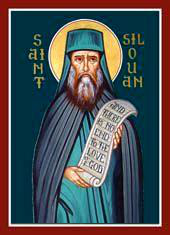
\includegraphics[width=0.2\linewidth]{img/521.jpg}
%~ \end{floatingfigure}
%~ 
%~ Будущий старец Силуан родился в крестьянской семье Тамбовской губернии в 1866 году, Призванный на военную службу в Петербург, он «умом пребывая на Афоне и на Страшном Суде», получает у св. праведного Иоанна Кронштадтского благословение на монашеский подвиг и в 1892 году становится послушником русского Пантелеимонова монастыря на Афоне.
%~ 
%~ Монашеские подвиги преподобного Силуана были тайными, но особую благодать, которая от него исходила, чувствовали все, от простых рабочих до церковных иерархов. 
%~ 
%~ После смерти старца, последовавшей в 1938 году, в Пантелеимонов монастырь стали приходить многочисленные письма, свидетельствующие о его небесном предстательстве за тех, кто обращался к нему с молитвой.

\newpage\section{myfig}
\setlength\intextsep{0pt}
\myfigr[0.15]{img/521.jpg}

Будущий старец Силуан родился в крестьянской семье Тамбовской губернии в 1866 году, Призванный на военную службу в Петербург, он «умом пребывая на Афоне и на Страшном Суде», получает у св. праведного Иоанна Кронштадтского благословение на монашеский подвиг и в 1892 году становится послушником русского Пантелеимонова монастыря на Афоне.

Монашеские подвиги преподобного Силуана были тайными, но особую благодать, которая от него исходила, чувствовали все, от простых рабочих до церковных иерархов. 

После смерти старца, последовавшей в 1938 году, в Пантелеимонов монастырь стали приходить многочисленные письма, свидетельствующие о его небесном предстательстве за тех, кто обращался к нему с молитвой.

\end{document}
